% !TEX root = main.tex
\documentclass[a4paper, UKenglish, 11pt]{uiomaster}
\usepackage{lipsum}
\usepackage[subpreambles=true]{standalone}
\usepackage{graphicx}


\begin{document}

\chapter{Creating EEG Data}
In preparation for the application of neural networks to address the inverse problem, the acquisition of a substantial and appropriate EEG dataset is essential. This chapter focuses on utilizing the New York Head model in conjunction with the current dipole approximation to construct biophysically realistic EEG data.

\section{Simulation of EEG Signals from single dipoles}
\rednote{Include range of x, y, z values and maybe eeg ?}
% The New York Head model and its  were made available for reuse in the {\tt h5py} Python package.
The New York Head model and its lead field matrix are integrated into the Python module LFPy. Within LFPy, we use the \texttt{NYHeadModel} class to calculate EEG signals originating from a current dipole moment $p$. The current dipole moments of the LFPy package are expressed in terms of nA$\mu$m, while the EEG signals derived from the NYHM are recomputed into units of mV. For more information about the LFPy module, we refer the reader to Hagen, Næss, Ness and Einevoll (2018) \cite{LFPy}.

The lead field matrix of the NYHM comprises 74,382 discrete points, each corresponding to possible locations for dipole sources. In the context of simulating EEG measurements, the procedure commences with the random selection of positions from these points to serve as the locations for placing dipoles. Each simulated EEG sample entails a solitary dipole positioned at one of the randomly chosen locations. As the primary objective is to address the inverse problem, maintain uniform magnitudes for the dipole signals, as their variation is not of primary concern. By setting these magnitudes to $10^7$ nA $\mu$m, the resulting EEG measurements span a range of approximately -1 to 1 $\mu$V.

\rednote{Vise tilbake til forrige kapittel med dipolorientering?}
To ensure that the dipole orientations are predominantly aligned with the depth direction of the cortex, a rotation procedure is employed for each dipole moment, orienting it perpendicular to the cerebral cortex. Note that aligning the dipole orientations perpendicularly to the cortex does not always lead to the dipole's normal vector pointing directly outward toward an EEG electrode. This variability arises due to the complex folding patterns found in the human cortex. In certain cases, when a dipole is located within a sulcus, the electrical signal it generates may follow the contour of the sulcus and enter deeper into the cortex. Consequently, the EEG signal must traverse a more extended path before ultimately reaching an EEG electrode \cite{naess2021biophysically}.

The NYHM generates EEG signals as time series data, reflecting the structure of real-world measurements. As a result, the inherent format of EEG data deviates from a one-dimensional representation, instead adopting a matrix configuration of 231 times 1601 dimensions. In this arrangement, 231 values represent measurements from scalp recording electrodes, with 1601 time steps marking the temporal progression. However, as mentioned in the preceding chapter, EEG analysis often centers on specific frequency components within each temporal instance of measurement. This practice effectively reduces the multidimensional EEG data and eliminates less relevant data points.

In our analysis, we have adopted a one-dimensional data approach to pinpoint sources of neural activity. This discrepancy from conventional practices, which involve extracting diverse frequency spectra and analyzing time series to identify anomalies, offers simplification and computational efficiency. Additionally, this transition is well-suited to our simulated data, which lacks confusing signals from brain activity or unclear background noise, simplifying the data preparation before being fed into a neural network. Rather than conducting a time series analysis with frequency extraction, we focus on data from a static dipole representing a chosen time point. This approach results in a one-dimensional EEG signal that effectively encapsulates insights into the spatial distribution of EEG patterns and their relationship with specific dipole source locations within the cerebral cortex.
\rednote{Add plot of NYHM timeseries data?}


\section{Noise}
Experimental EEG recordings inevitably contain noise, which can interfere with the accurate analysis of brain activity. \emph{Artifacts}, which are signals recorded by EEG but originating from sources other than neuronal communication, pose a particular challenge in real-world data. Some artifacts can mimic genuine epileptiform abnormalities or seizures, underscoring the importance of identifying and distinguishing them from true brain waves \cite{sazgar2019eeg}.

Artifacts can be classified into two categories based on their origin. \emph{Physiological artifacts} arise from the patient's own physiological processes, including ocular activity, muscle activity, cardiac activity, perspiration, and respiration. \emph{Technical artifacts}, on the other hand, originate from external factors such as cable and body movements or electromagnetic interferences \cite{bitbrain}.

Filtering techniques are commonly employed to remove artifacts from EEG recordings prior to analysis. However, in the case of simulated EEG data, the need for artifact removal is eliminated as the data inherently do not contain noise. Simulated EEG data can be considered as pre-filtered and preprocessed, ensuring a high signal-to-noise ratio (SNR) \cite{wiki-snr}. Nevertheless, to ensure the data aligns with real-world scenarios and accounts for other technical considerations which we will come back to later, it is necessary to introduce noise to the data before feeding it into the neural network.

In our approach, we recognize that the introduction of noise to the simulated EEG data is an essential step to enhance the robustness of the trained neural network and ensure its ability to handle real EEG recordings effectively. Since the specific characteristics and quantity of noise have not been the primary focus of our study, we have opted for a straightforward approach. Our final dataset incorporates normally distributed noise with a mean of 0 and a standard deviation equal to 10$\%$ of the standard deviation observed in the simulated EEG recordings. By introducing this noise, we introduce random variations around each data point while preserving the overall normalization properties of the dataset.

\begin{figure}[!htb]
    \centering
    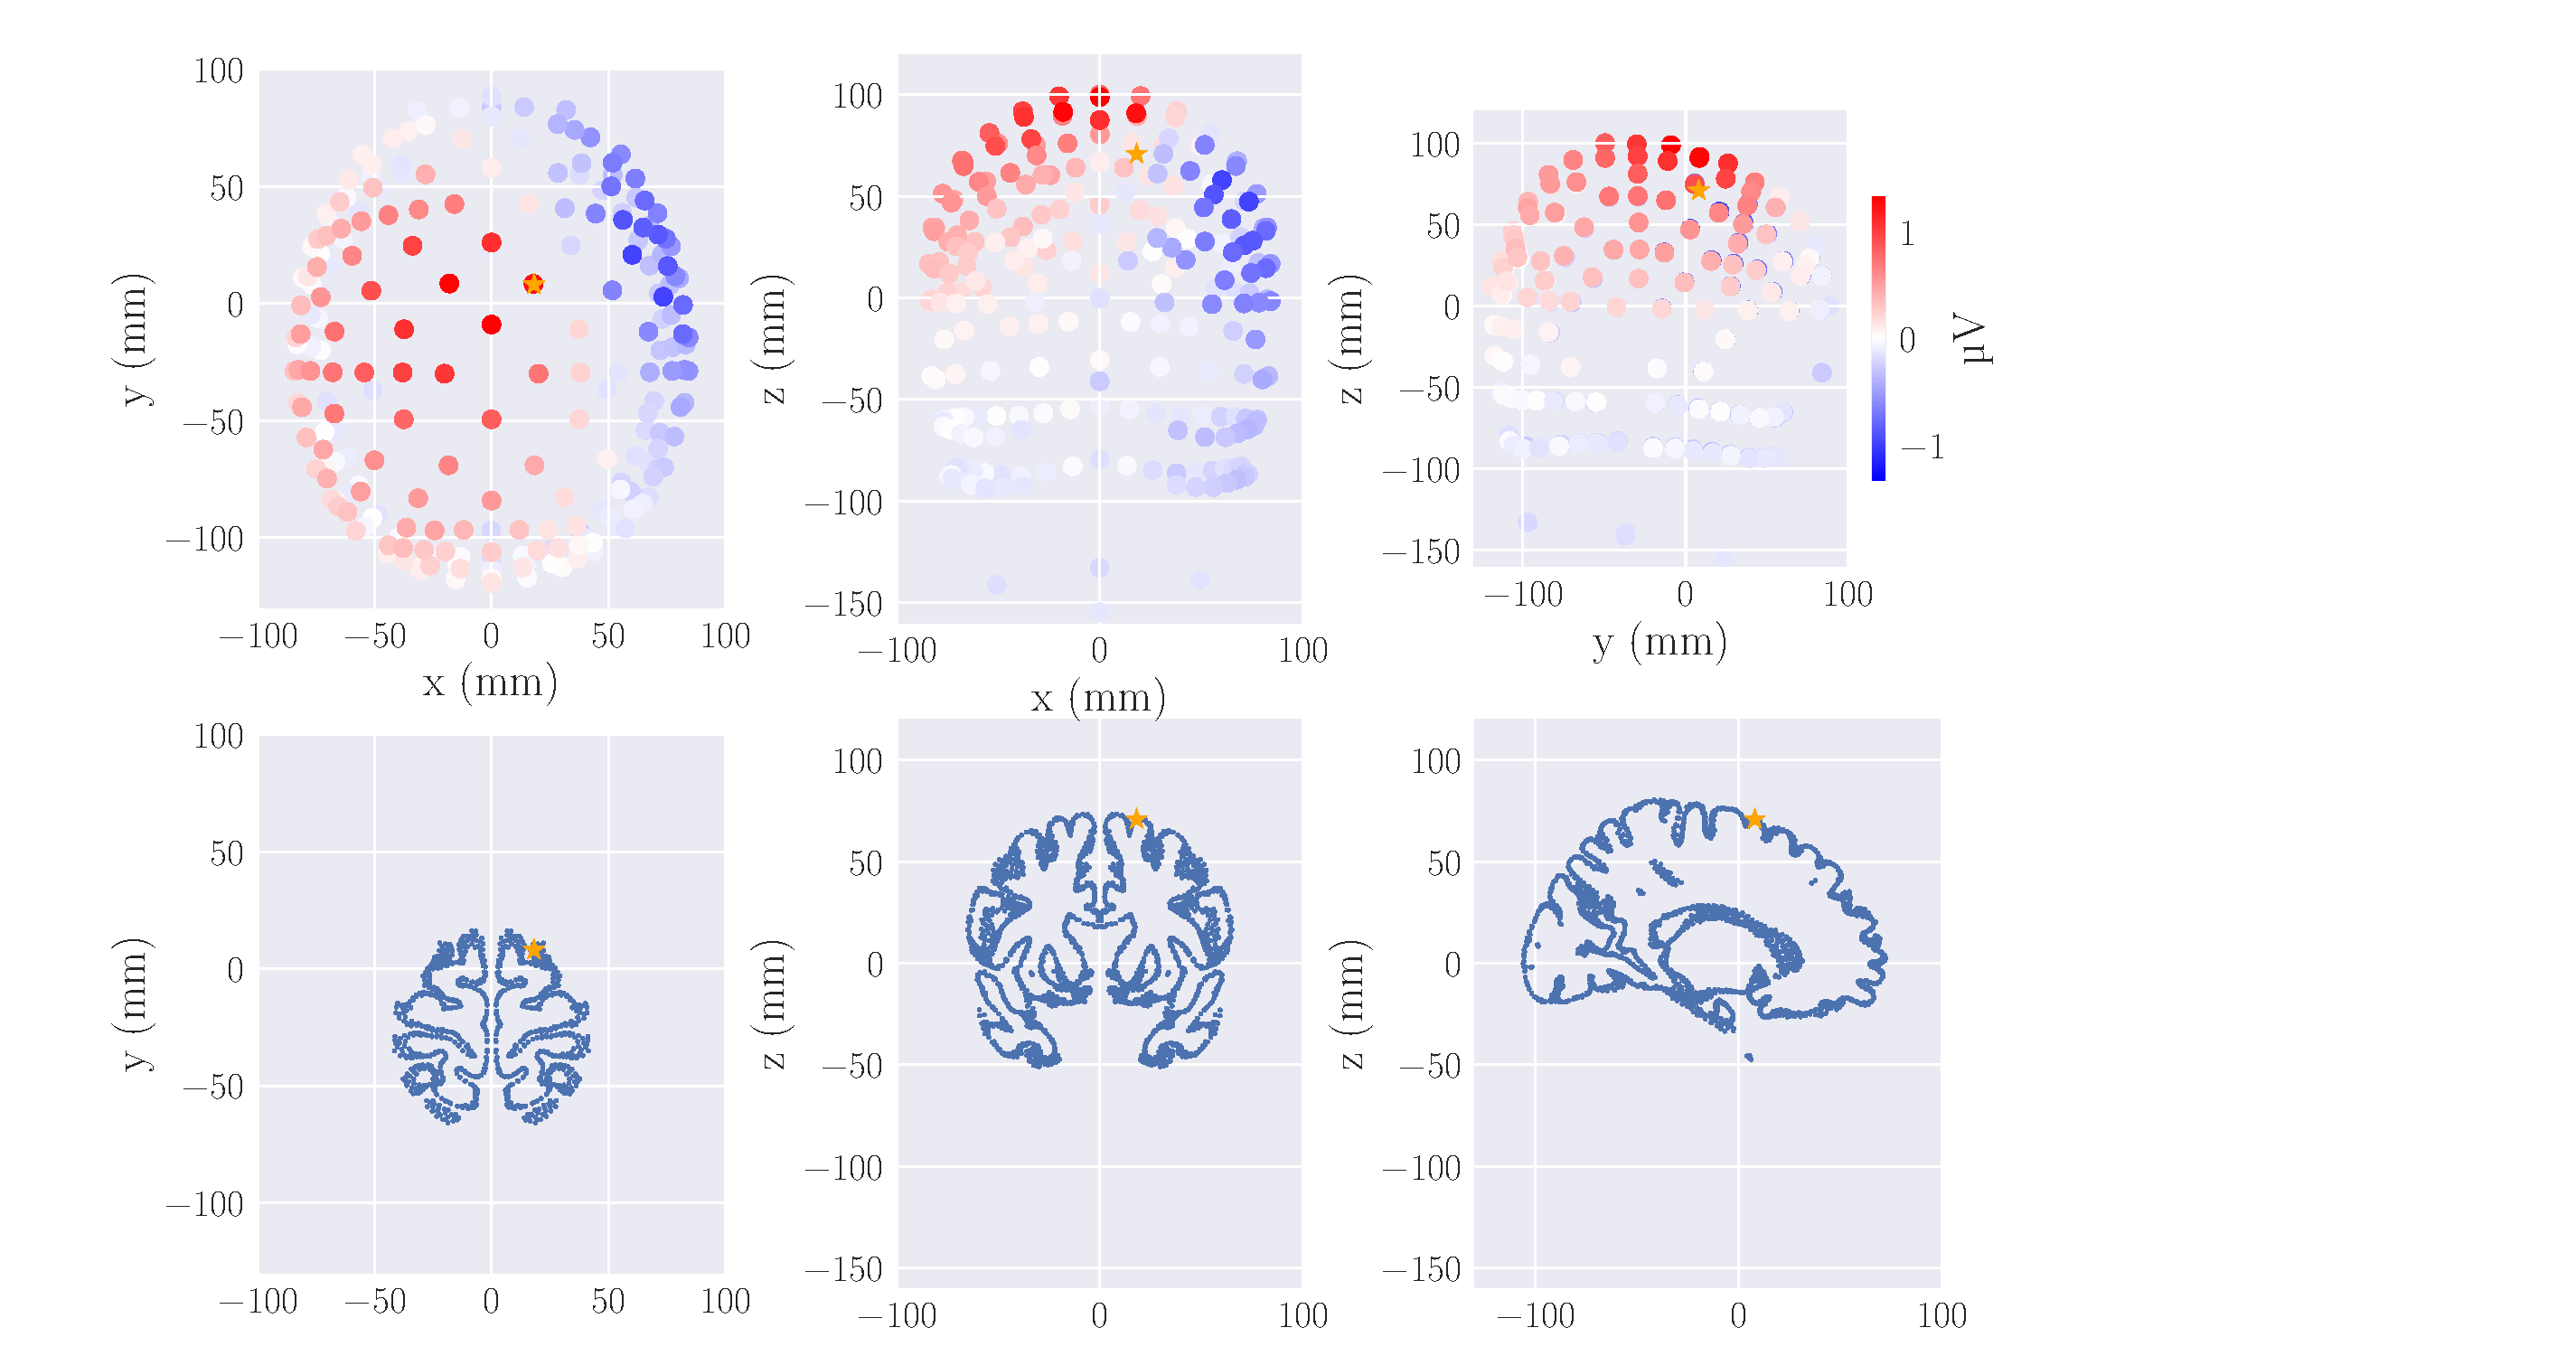
\includegraphics[width=\linewidth]{figures/simple_example.pdf}
    \caption{EEG for a sample containing one single current dipole source at a random position within the celebral cortex. As for all samples within the data set, 10 percent of normally distributed noise has been added to the original signal. The EEG measure is seen from both sides (x-, z-plane and y-, z-plane) and above (the x-, y-plane). EEG electrode locations are presented as filled circels, where the color of the fill represents the magnitue of the measured signal for the given electrode. The position of the current dipole moment is marked with a yellow star.}
    \label{fig:eeg_field_1_dipole_example}
\end{figure}

\subsection{Final Dataset}
The final dataset comprises 70, 000 rows, where each row corresponds to a single sample or fictive patient. Within the dataset, there are 231 columns representing the features, which denote the EEG measurements recorded at each electrode - a configuration directly derived from the NYHM. In practice, the data consists of two separete files holding pairs of EEG data and corresponding target data, where x-, y- and z coordinates of different dipole sources are the answer keys.

Figure \ref{fig:eeg_field_1_dipole_example} presents an example of the input EEG data for a single sample, with 10$\%$ noise added. The EEG result obtained from the specific sample contains a solitary current dipole source positioned randomly within the cerebral cortex. The prominent dipolar pattern in the figure indicates that the dipole is located within a sulcus. In the figure the EEG measure is visualized from multiple perspectives, including the x-z plane, y-z plane, and the x-y plane. The electrode locations are represented by filled circles, with the color of the fill indicating the magnitude of the measured signal at each electrode. The position of the current dipole moment is denoted by a yellow star. As indicated by the colorbar in the figure, the EEG signal for the specific sample ranges from -1 to 1~$\mu$V, which is the range that the simulated EEG data for all samples will fall within.



% Before being feed to the DiLoc network for training, the data is splitted into train, validation and test parts. The train- and validation data are the batches of the data set that the network uses during training. Out of the 70 000 samples in the final dateset, 50000 is set off to the purpose of train and validation data. Out of these 50000 sampes, randomly selected 80 percent of the rows are put into the training set. The remaining 20 percent operates as the validation set, which is useful in order to prevent the network to overfit during training. The test set which contains the final 20 000 samples will be used after the training prosess for the purpose of testing how well the model generalizes to new, unseen data.
%
% Prior to being fed into the DiLoc network for training, the dataset was splittied into distinct segments: the train, validation, and test sets. This partitioning is vital for assessing and optimizing the network's performance. Among the 70 000 samples in the final dataset, 50 000 samples are designated for the train and validation data. To ensure a representative and unbiased allocation, 80 percent of these 50 000 samples are randomly assigned to the training set. This training set serves as the core data that the network utilizes during the training process. The remaining 20 percent of the 50 000 samples form the validation set. This set plays the role in preventing overfitting, the phenomenon where the network becomes excessively attuned to the training data and consequently performs poorly on new data. By independently evaluating the model's performance on the validation set throughout training, we can fine-tune the network's parameters to achieve better generalization to unseen data. Once the network completes its training process, the test set comes into play. Comprising 20 000 samples, the test set serves as the benchmark for assessing the model's ability to generalize and make accurate predictions on new data instances. By adhering to this rigorous train-validation-test data partitioning, we ensure a robust evaluation of the DiLoc model's performance and its capacity to effectively handle real-world scenarios with previously unseen data.



\end{document}